%% JDSA Stage 3 scientific restructuring; baseline and immutable evidence preserved.

\documentclass[pdflatex,iicol,sn-basic,Numbered]{sn-jnl}

\usepackage{graphicx}
\usepackage{multirow}
\usepackage{amsmath,amssymb,amsfonts}
\usepackage{booktabs}
\usepackage{tabularx}
\usepackage{algorithm}
\usepackage{algorithmicx}
\usepackage{algpseudocode}
\usepackage{xurl}
\usepackage{microtype}
\usepackage{xr-hyper}
\usepackage{hyperref}
% Full URL/DOI links need no redundant "URL" label.
\providecommand{\urlprefix}{}
% Avoid duplicate caption destinations in the preserved Springer template.
\hypersetup{hypertexnames=false,
  pdftitle={Retrieval-Assisted Scalar Grounding for Natural-Language Optimization: A Diagnostic Study},
  pdfauthor={Soroush Vahidi},
  pdfsubject={Diagnostic study of retrieval-assisted scalar grounding},
  pdfkeywords={natural language processing, optimization modeling, information retrieval, semantic grounding},
  pdflang={en-US}}

\usepackage{orcidlink}
\raggedbottom

% Use standard PDF destinations in the corrected local companion document.
\externaldocument[S-]{supplement}[ESM_1.pdf]
\begin{document}

\title[Retrieval-Assisted Scalar Grounding]{Retrieval-Assisted Scalar Grounding for Natural-Language Optimization: A Diagnostic Study}

\author*[1]{\fnm{Soroush} \sur{Vahidi}\,\orcidlink{0000-0003-1934-6282}}\email{sv96@njit.edu}

\affil*[1]{\orgdiv{Department of Computer Science, Ying Wu College of Computing}, \orgname{New Jersey Institute of Technology}, \orgaddress{\street{University Heights}, \city{Newark}, \state{NJ}~\postcode{07102-1982}, \country{USA}}}

\abstract{Retrieval and structural checks can make natural-language optimization outputs appear usable even when numerical grounding is incomplete. We examine this diagnostic gap through three questions: fixed-catalog schema identification, the validity of coverage/type readiness as a numerical check, and the mechanisms underlying grounding outcomes. On 331 NLP4LP benchmark queries and 335 schema documents, term frequency--inverse document frequency retrieval and a pretrained dense encoder identify the target schema for 301 and 313 queries. Ratio-aware lexical grounding passes coarse readiness on 265 queries, but only seven meet the complete stored-reference scalar-tolerance criterion: 2.64\% of ready outputs. A mutually exclusive residual partition distinguishes retrieval, coverage, type, and numerical failures. Six grounding procedures under fixed retrieval yield between seven and 46 complete successes, with candidates, scoring, abstention, and decoding changing together. A separate 49-query frozen-score assignment study improves exact slot counts without increasing the five whole-instance tolerance successes, limiting attribution to search. The methodological contribution is joint reporting of retrieval, readiness, and complete scalar agreement with explicit assistance, denominators, and evidence boundaries. Reference-derived inventories and benchmark exposure restrict the findings to assisted grounding. Supplementary relationship judgments and author contrasts assisted by artificial intelligence illustrate semantic limits without establishing accuracy. A versioned public release supports saved-record reanalysis; missing historical predictions and restricted originals prevent full experimental reproduction.}

\keywords{natural language processing, optimization modeling, knowledge representation, information retrieval, semantic grounding, intelligent information systems}

\maketitle
% Apply after maketitle, which resets the template URL font.
% Literal URL characters remain copyable; xurl supplies column-safe breaks.
\urlstyle{tt}


\bmhead{Acknowledgements}

The author thanks his mother for emotional support, Professor Ioannis Koutis for academic guidance, NJIT for Wulver computing access, and Anders Borum for complimentary Secure ShellFish access. Cohere Labs Catalyst, Google Cloud Research Credits and io.net supported the author's broader research; their use for this study's experiments is not established. Study-specific educational credits and in-kind support are distinguished in Statements and Declarations.

\section{Introduction}
Natural-language optimization interfaces must connect a problem's quantities to the appropriate parameters and mathematical roles. Retrieving a suitable template and filling its slots provide complementary parts of this structure, but neither operation alone establishes that the numerical mapping expresses the intended problem. A capacity and a cost may share a value, and reversing a bound can preserve both the number and its type.

Entity extraction, structured representations, and formulation generation address different parts of this translation \cite{ramamonjison2022autoformulation,ramamonjison2023nl4opt,kadioglu2024ner4opt,ahmaditeshnizi2024optimus_icml}. Database interfaces distinguish schema elements from their links to textual values \cite{deng2021strug,wang2020ratsql}, and Text2Opt-Bench explicitly separates modeling from data binding \cite{gao2026models}. Building on these established concerns, we ask which intermediate measurements reveal numerical binding failures and which favorable measurements can coexist with incomplete numerical results.

Retrieval-assisted scalar grounding provides an inspectable setting for this diagnosis. A retriever selects a document from a fixed catalog, and an existing deterministic procedure assigns extracted numerical mentions to scalar slots, producing a partial parameter mapping. The benchmark supplies reference-derived inventory information and includes all target schemas (Section~\ref{subsec:assistance-setting}). This setting supports analysis of intermediate checks under supplied structure, rather than evaluation of autonomous model formulation.

Three research questions organize the paper:
\begin{enumerate}
\item \textbf{RQ1---Schema retrieval:} How well does fixed-catalog retrieval identify the benchmark's target schema?
\item \textbf{RQ2---Diagnostic validity:} How often do structural coverage and type-readiness checks conceal failures of complete numerical grounding?
\item \textbf{RQ3---Grounding mechanisms:} What do matched grounding comparisons and frozen-score assignment controls reveal about candidate availability, scoring, abstention, and search?
\end{enumerate}

The 331-query NLP4LP analysis jointly reports schema hits, coarse readiness, and agreement across every required stored-reference scalar, then partitions residual failures. It includes a comparison of six complete grounding procedures on that frame and a separate 49-query assignment control that fixes candidate pools and scores within decoder comparisons. Neither population is an independent confirmatory sample.

The contributions are correspondingly focused:
\label{subsec:intro_contributions}
\begin{enumerate}
\item A diagnostic protocol for reference-assisted supplied-slot grounding that jointly reports retrieval, coverage/type readiness, and complete stored-reference scalar agreement with explicit input assistance and denominators.
\item A saved-record analysis of the 331-query benchmark that quantifies the readiness--grounding discrepancy through a mutually exclusive residual partition while preserving conditional Exact20 populations.
\item A distinction between whole-procedure comparisons and frozen-score assignment controls that clarifies what retained candidate, scoring, and search records can explain, supported by a versioned reanalysis package with explicit reconstruction limits.
\end{enumerate}

The contribution lies in applying these diagnostics to supplied-slot grounding, not in priority for component-level evaluation or a new retrieval or matching algorithm. Semantic fidelity requires further validation: supplementary relationship judgments and contrasts prepared by the author with artificial intelligence (AI) assistance illustrate this boundary without providing independent semantic gold or provider-performance claims. Online Resource 1 preserves the other formulation, extraction, and historical auxiliary results under their own protocols.

Section~\ref{sec:related_work} places this diagnostic approach in the context of grounding and formulation research. Sections~\ref{sec:task} and~\ref{sec:methodology} define the endpoints and comparisons; Section~\ref{sec:experiments} addresses RQ1--RQ3, and Section~\ref{sec:discussion} interprets the findings and limitations.

\section{Related Work}
\label{sec:related_work}
\subsection{Structured Grounding and Numerical Binding}
\label{subsec:rw_binding}
StruG learns column grounding, value grounding, and column--value mapping for text-to-SQL \cite{deng2021strug}; RAT-SQL encodes schema relations and linking \cite{wang2020ratsql}. Quantity interpretation similarly associates values with units and concepts \cite{almasian2023cqe,roy2017udg}. These studies distinguish element identification from linking to textual evidence. Their learned representations do not implement the supplied-slot protocol evaluated here.

Text2Opt-Bench studies solver-verified optimization problems with increasing numerical data, even when formulation structure remains simple \cite{gao2026models}. Its BIND interventions distinguish oracle-assisted data externalization from trained binding specialists; the study also documents failures of an untrained two-stage pipeline. We do not reproduce these interventions. Our narrower question concerns complete stored-reference scalar agreement among outputs that pass coverage/type checks and the explanations supported when assignment inputs and scores are fixed. The scaling and intervention results are therefore not directly comparable to these exposed-catalog conditional diagnostics.

\subsection{Formulation Systems and Evaluation Endpoints}
\label{subsec:rw_llm_generation}\label{subsec:rw_retrieval_memory}
Optimization systems also differ in their outputs and evaluation endpoints. NL4Opt and Ner4Opt examine optimization-related extraction and representations \cite{ramamonjison2023nl4opt,kadioglu2024ner4opt}. OptiMUS and PaMOP generate formulations or solver code with feedback \cite{ahmaditeshnizi2024optimus_icml,pan2025pamop}, whereas OptMATH, ORLM, and DeepOR develop data or trained modeling systems \cite{lu2025optmath,huang2025orlm,xiao2026deepor}. Retrieval for code generation, as in OPT2CODE, differs from selecting the parameter inventory itself \cite{ahmed2025opt2code}. Online Resource 1, Table~\ref{S-tab:comparison_landscape} and Section~\ref{S-app:related-context}, provide the broader system context. End-to-end outcomes from these systems cannot substitute for scalar-binding measurements.

A related diagnostic perspective appears in Refai and Ahmed's component-level evaluation of generated formulations, including decision-variable and constraint precision/recall and constraint/objective root mean squared error \cite{refai2026component}. OPT-Engine varies optimization-problem complexity to examine formulation and solving limitations, including constraint formulation \cite{chen2026optengine}. Within our reference-assisted scalar inventory, we condition complete stored-reference agreement on readiness and use ordered gate accounting and fixed-score decoder comparisons to delimit failures and their attribution.

The role of search also depends on the task. OptMATH synthesizes modeling data through back-translation and forward checking \cite{lu2025optmath}; our external extraction check evaluates neither that framework nor full-pipeline transfer. Autoformulation combines large language model (LLM)-guided Monte Carlo tree search with symbolic pruning over formulations \cite{astorga2025autoformulation}, including modeling decisions outside our supplied-slot assignment controls. These distinctions describe task scope, not empirical comparisons with either system.

Structural validity and semantic validation require different checks. Constrained semantic-role inference and PICARD impose structural restrictions \cite{punyakanok2004ilp,scholak2021picard}, whereas EquivaMap checks mappings between formulations that preserve feasibility and optimality \cite{zhai2025equivamap}. Our stored-scalar test establishes neither formulation equivalence nor fidelity to the source description; these stronger endpoints delimit what a positive diagnostic result means.

\subsection{Methodological Position}
\label{subsec:rw_position}
For reference-assisted supplied slots, we combine complete stored-reference agreement, ordered gate accounting, explicit conditional populations, and controlled attribution from saved records. Classical maximum-sum assignment \cite{kuhn1955assignment}, existing retrievers, and existing grounders serve as diagnostic instruments. The six-method comparison holds retrieval and queries fixed while changing several grounding components; the separate factorial holds scores fixed within decoder comparisons. This design distinguishes procedure-level gains from search effects and readiness from formulation correctness.

\section{Problem Setting and Evaluation Framework}
\label{sec:task}
\subsection{Problem Formulation}
\label{subsec:method_problem}

Given a query, the system returns a top-1 catalog schema and a partial mapping of its scalar parameters \cite{nlp4lp_dataset}. Schema retrieval ranks $\mathcal{S}=\{s_1,\dots,s_M\}$ and returns
\begin{equation}
\hat{s}=\arg\max_{s \in \mathcal{S}} \mathrm{score}(q,s).
\label{eq:top1_schema}
\end{equation}
Parameter instantiation extracts numerical mentions and assigns them to scalar slots of $\hat{s}$ using deterministic rules. Incorrect retrieval can produce an inappropriate eligible slot set even when the query contains usable numerical evidence.

A \emph{schema} comprises the retrieved template and its parameter structure. The core task excludes complete program synthesis and list-, vector- or dictionary-valued recovery. Numerical grounding is rule-based; optional dense retrieval uses a pretrained encoder.

Let $K_G(q)$ contain keys whose gold values are numeric scalars (integers or floats, excluding booleans). Let $P_{\mathrm{all}}(\hat{s})$ contain \emph{all} keys in the predicted schema's parameter-metadata dictionary, with a fallback to all keys in its reference parameter record when the parameter metadata is not a dictionary. This construction does not first filter entries by scalar shape. The benchmark constructs assignments on the eligible set
\begin{equation}
E(q,\hat{s}) = K_G(q) \cap P_{\mathrm{all}}(\hat{s}).
\label{eq:eligible_slots}
\end{equation}
Gold scalar status therefore filters the slot inventory \emph{before} assignment: gold keys affect both prediction construction and evaluation, although the mention-selection rule does not receive gold numerical magnitudes. Let $y_q : K_G(q) \to \mathbb{R}$ be the gold map and $\hat{y}_{q}$ the partial assignment on $A(q) \subseteq E(q,\hat{s})$; masked inputs may leave a raw unknown token rather than a numeric value. Retrieval quality measures top-1 schema match, whereas downstream quality measures how well eligible scalars are filled from text.

\subsection{Evaluation Inputs and Reference Assistance}
\label{subsec:assistance-setting}

The main four-arm and matched-baseline experiments use reference information during prediction, not only for scoring. They are \emph{gold-assisted}: the expected scalar count and slot identities depend on $K_G(q)$ before value selection, so slot-name type heuristics also operate on reference-derived names. The numeric selector does not receive gold magnitudes, objective coefficients, or constraint identities as separate targets. This restriction on the selector's inputs does not make the full pipeline autonomous.

The catalog is also benchmark-derived. Its builder pairs each test description with the same record's parameterized description, falling back to its description and a metadata signature. The retained catalog contains 331 test-record documents plus four fillers; all 331 target IDs are present, and six query--target texts match exactly. This is known-template identification rather than held-out template generation. Fitting an index without supervision does not establish independence from the evaluation source.

The later joint/factorial controls remove the query-specific gold-key filter but retain the selected reference template's slot names, shapes, and descriptions, with types inferred heuristically from names. These \emph{partially assisted} controls also use any available parameter relations from that template and measure assignment conditional on supplied structure. The 20-case execution check is gold-assisted: it additionally retains reference code and unfilled scalar/structured values. Online Resource 1, Section~\ref{S-app:reproduction}, details these boundaries and distinguishes prediction reconstruction from aggregation. The saved records identify neither an autonomous formulation score nor an adjustment that would estimate one from these conditional scores.

\subsection{Inference Dependencies and Practical Scope}
\label{subsec:inference-dependencies}
The lexical path uses catalog-fitted term frequency--inverse document frequency (TF--IDF), cosine ranking, numerical parsing, and typed assignment, without generative-model calls or task-specific neural training. Optional BGE-M3 retrieval uses a pretrained encoder; the external generation and relationship studies use model services separately. Cached dependencies and metadata permit local lexical inference, but no comparative cost, privacy, or reliability benefit is measured. Historical replay also requires the run's ordering and environment (Section~\ref{subsec:limitations}).

\subsection{Metric Levels and Denominators}\label{subsec:metrics}
\textit{Schema R@1} is $N^{-1}\sum_{i=1}^N H_i$, where $H_i=\mathbf{1}[\hat{s}_i=s_i^*]$ and $N=331$. For downstream metrics, let $E_i=E(q_i,\hat{s}_i)$ and let $A_i\subseteq E_i$ denote the assigned slots. Let $T_i\subseteq A_i$ contain assignments accepted by the implemented coarse-type compatibility predicate. Compatibility is broader than literal type equality: in addition to same-type matches, integer mentions are accepted for float slots, and integer or float mentions for currency slots. Expected types are inferred heuristically from slot names, not from annotated semantic roles. Define
\begin{equation}
\begin{gathered}
c_i=\begin{cases}|A_i|/|E_i|,& |E_i|>0,\\0,& |E_i|=0,\end{cases}
\\[3pt]
\textit{Coverage}=\frac{1}{N}\sum_{i=1}^N c_i,
\end{gathered}
\label{eq:coverage}
\end{equation}
\begin{equation}
\begin{gathered}
t_i=\begin{cases}|T_i|/|A_i|,& |A_i|>0,\\0,& |A_i|=0,\end{cases}
\\[3pt]
\textit{TypeMatch}=\frac{1}{N}\sum_{i=1}^N t_i.
\end{gathered}
\label{eq:typematch}
\end{equation}
Coverage and TypeMatch in Eqs.~\eqref{eq:coverage} and~\eqref{eq:typematch} are \emph{macro-averages over queries}, with zero-denominator queries contributing zero. Separate type-stratified diagnostic files instead pool slots by type. Abstention leaves a slot unfilled and reduces coverage; TypeMatch conditions on assigned slots within each query before averaging across all queries. Missing retrieval yields an empty eligible set and zero coverage and type score. A masked mention can count as assigned without a comparable numerical value, but its implemented unknown type fails the coarse-type predicate.

For a schema-hit query, let $C_i\subseteq A_i$ contain slots with both a numeric prediction and numeric gold value. For each comparable slot,
\begin{equation}
 e_{i,s}=\frac{|\hat{y}_{i,s}-y_{i,s}|}{\max(1.0,|y_{i,s}|)}.
\label{eq:bounded_error}
\end{equation}
A slot passes the inclusive tolerance rule if $e_{i,s}\leq0.20$: absolute error at most $0.20$ for $|y|<1$, otherwise relative error at most $20\%$. No additional type gate is imposed on this numerical comparison. With $J=\{i:H_i=1,\ |C_i|>0\}$,
\begin{equation}
\begin{gathered}
x_i=\frac{1}{|C_i|}\sum_{s\in C_i}\mathbf{1}[e_{i,s}\leq0.20],
\\[3pt]
\textit{Exact20 (on hits)}=\frac{1}{|J|}\sum_{i\in J}x_i.
\end{gathered}
\label{eq:exact20}
\end{equation}
The comma-separated values (CSV) field \texttt{exact20} stores $x_i$, a slot fraction rather than a whole-query indicator. It is blank on schema misses or when $C_i$ is empty. These queries are excluded from the reported Exact20 mean, not assigned zero; an empty $J$ is reported as unavailable. The main-table denominators are 291, 291, 303, and 320 \emph{queries} for TF--IDF baseline, TF--IDF ratio-aware, BGE-M3, and Oracle. Because missing numerical predictions are not counted as errors in this conditional metric, abstention can improve Exact20 while lowering coverage. The method-dependent subsets therefore do not support an unconditional accuracy ranking.

\textit{InstantiationReady} retains its historical metric identifier for reproducibility and is described here as \emph{coarse readiness}:
\begin{equation}
\begin{gathered}
\mathit{InstantiationReady}_i\\[2pt]
=\mathbf{1}[c_i\geq0.8\ \wedge\ t_i\geq0.8].
\end{gathered}
\label{eq:instantiation_ready}
\end{equation}
The score in Eq.~\eqref{eq:instantiation_ready} is averaged over all $N$ queries. It checks neither schema correctness nor numerical values and can tolerate unfilled or incompatible slots. StrictInstantiationReady (strict readiness) additionally requires $H_i=1$, but still does not check values.
\begin{equation}
\begin{gathered}
\mathit{StrictInstantiationReady}_i\\[2pt]
= \mathbf{1}[H_i=1\ \wedge\ c_i\geq0.8\ \wedge\ t_i\geq0.8].
\end{gathered}
\label{eq:strict_instantiation_ready}
\end{equation} Empty eligible or assigned sets fail both readiness criteria. Thus an $80\%$ coarse-readiness rate is not an $80\%$ correct-instance rate.


To state the complete endpoint explicitly, let $F_i^G$ indicate a schema hit with every required scalar assigned, comparable, type-compatible and within tolerance:
\begin{equation}
\begin{split}
F_i^G=\mathbf{1}[\,&H_i=1,\ K_G(q_i)\ne\varnothing,\\
&A_i=C_i=T_i=K_G(q_i),\\
&\max_{s\in K_G(q_i)}e_{i,s}\leq0.20\,].
\end{split}\label{eq:full-scalar}
\end{equation}
An empty required set fails this criterion. Unlike conditional Exact20, $F_i^G$ cannot reward missing keys or incomparable values. Write $I_i$ and $S_i$ for ordinary and strict readiness, and $F^G$, $S$ and $I$ for the corresponding query sets. Since $F^G\subseteq S\subseteq I$, we also report
\begin{equation}
\rho_I=\frac{\sum_i F_i^G}{\sum_i I_i},\qquad
\rho_S=\frac{\sum_i F_i^G}{\sum_i S_i}.
\label{eq:conditional-agreement}
\end{equation}
These fractions describe agreement among a method's ready outputs; a zero denominator would be reported as unavailable. They are not semantic precision estimates: the denominators are method-dependent subsets of the same exposed benchmark. These descriptive summaries receive no independence-based uncertainty interval or new hypothesis test.

\section{Methods and Experimental Setup}
\label{sec:methodology}\label{sec:method}
\subsection{RQ1: Retrieval Protocol}
\label{subsec:method_retrieval}\label{subsec:exp_setup}
We use the 331 historically designated NLP4LP test queries \cite{nlp4lp_dataset,ahmaditeshnizi2024optimus_icml}, each with one target schema in the fixed 335-document catalog (Section~\ref{subsec:assistance-setting}). The variants are \emph{orig} (full text), \emph{noisy} (controlled lexical corruption and numerical masking), and \emph{short} (first sentence). The test designation does not imply an untouched evaluation set because the benchmark was used repeatedly during development.

We compare BM25, TF--IDF cosine retrieval, latent semantic analysis (LSA), and the pretrained BGE-M3 encoder \cite{robertson2009bm25,pedregosa2011sklearn,deerwester1990lsa,chen2024m3embedding}; Table~\ref{S-tab:retrieval_backbones} summarizes their representations. Classical indexes fit the catalog without query-label supervision, and only the top-1 schema enters grounding. Uniform random retrieval gives the theoretical reference $1/335\approx0.0030$. Oracle selection substitutes the target schema as a control; it is not a guaranteed upper bound on other grounders. BGE reporting metadata specifies float32, L2-normalized 1024-dimensional embeddings and cosine similarity, but does not authenticate the executed device or complete environment. Dataset tooling uses Hugging Face \texttt{datasets} \cite{lhoest2021datasets}.

\subsection{RQ2: Grounding and Endpoint Diagnosis}
\label{subsec:method_instantiation}\label{subsec:method_design}
The rule-based extractor recognizes integers, decimals, written numbers, fractions, percentages, currency-like forms, and comma-separated magnitudes. Ratio-aware extraction adds supported multiplicative words such as ``twice'' and ``triple''; masked tokens remain numerically unknown. Surface cues assign percent, integer, currency, or float types to mentions, while parameter-name heuristics determine expected slot types. Eligible slots follow Eq.~\eqref{eq:eligible_slots}, and compatibility follows Section~\ref{subsec:metrics}.

Typed greedy visits the run's slot order and assigns an unused indexed mention:
\begin{equation}
t_i^*=\arg\max_{t\in\mathcal T\setminus\mathcal U_{i-1}}\mathrm{compat}(p_i,t).
\label{eq:typed_assignment}
\end{equation}
Compatibility ranks candidates by coarse type preference, absolute magnitude, and raw surface text, retaining source order for remaining ties. Mention indices cannot be reused, but equal values at distinct occurrences remain distinct candidates. Slot iteration follows Python set order, so replay requires the historical interpreter/hash configuration. The headline configurations omit optional lexical role cues. Algorithm~\ref{alg:instantiation} and Figure~\ref{fig:instantiation-pipeline} describe this protocol.

\begin{algorithm*}[t]
\caption{Reference-assisted deterministic parameter instantiation without mention-index reuse.}
\label{alg:instantiation}
\small
\begin{algorithmic}[1]
\Require Query text $q$, predicted schema $\hat{s}$, gold scalar keys $K_G(q)$
\Ensure Slot--value mapping $A$
\State Extract numeric mentions $\mathcal{T}$ from $q$
\State Infer a coarse type for each mention in $\mathcal{T}$
\State Obtain parameter keys from schema $\hat{s}$
\State Set $\mathcal{P}=P_{\mathrm{all}}(\hat{s})\cap K_G(q)$; use the run's set iteration order
\State Infer an expected type for each slot in $\mathcal{P}$
\State Initialize assignments $A \leftarrow \emptyset$ and used-mention set $\mathcal{U}\leftarrow \emptyset$
\For{each slot $p_i \in \mathcal{P}$}
    \State Define candidate set $\mathcal{C}_i \leftarrow \mathcal{T} \setminus \mathcal{U}$
    \If{$\mathcal{C}_i = \emptyset$}
        \State \textbf{continue}
    \EndIf
    \State Score mentions in $\mathcal{C}_i$ using a deterministic slot--mention compatibility rule
    \State Select the highest-ranked mention $t_i^{*}$
    \State Assign $A[p_i] \leftarrow \mathrm{value}(t_i^{*})$ if numeric; otherwise retain its raw unknown token
    \State Update $\mathcal{U} \leftarrow \mathcal{U} \cup \{t_i^{*}\}$
\EndFor
\State \Return $A$
\end{algorithmic}
\end{algorithm*}

\begin{figure*}[t]
  \centering
  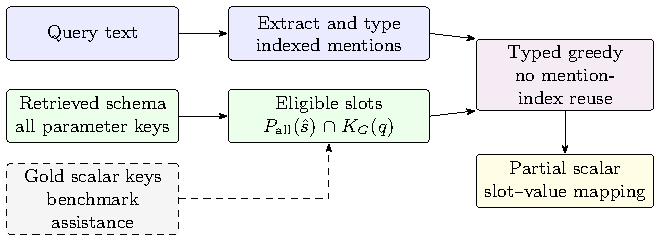
\includegraphics[width=0.90\textwidth]{Fig1.pdf}
  \caption{Historical typed-greedy instantiation with explicit reference assistance. Typed query mentions fill slots formed by intersecting predicted-schema metadata keys (with reference-key fallback) and gold scalar keys. Assignment consumes mention indices, not unique values. The later metadata-only factorial protocol uses a different inventory.}
  \label{fig:instantiation-pipeline}
\end{figure*}

The four headline arms are TF--IDF with baseline extraction, TF--IDF with ratio-aware extraction, BGE-M3 with ratio-aware grounding, and Oracle typed greedy. Their saved query metrics support the endpoints and ordered residual partition. Although the two ratio-aware retrieval arms use the same grounding implementation, their frozen assignments differ even on shared hits, so their numerical differences cannot all be attributed to retrieval. Core endpoints require no solver execution. Independent row-indicator and decimal set-intersection calculations verify the readiness-conditioned fractions from authenticated records.

\subsection{RQ3: Whole-Procedure and Frozen-Score Comparisons}
\label{subsec:method_controls}
Six existing procedures share all 331 original queries and TF--IDF retrieval: typed greedy, constrained assignment, maximum-weight matching, optimization-role repair, search-structured grounding, and semantic intermediate-representation (IR) repair. Candidates, context, scoring, abstention, and decoding can differ. Typed greedy and constrained assignment both prevent mention reuse and share ratio-aware patterns, but use different token/mention constructors; the other procedures retain their intrinsic enriched extractors. Methods were selected before this matched comparison, without additional tuning against its labels, although earlier benchmark exposure remains. The comparison therefore evaluates complete procedures rather than isolating the decoder.

The separate factorial holds candidates and edge-score matrices fixed within each decoder pair. It crosses two candidate constructors, three scorers, two decoders, and two mention-reuse policies: 24 cells on 49 primary queries and 277 scalar slots. Each pair shares canonical lexical slot order and a zero-score null option. The ordinal type-preference control explicitly cardinalizes preferences; it does not reconstruct every historical greedy decision. The remaining scorers use contextual scores with or without percent/currency marker bonuses. With unrestricted reuse and additive scores, independent per-slot maximization already solves the stated objective. One-to-one matching is thus a diagnostic restriction, not a general requirement of formulation.

The original collection contains 64 cases: 49 primary, 12 development, one overlap-reconciliation, and two reference-only. Query 291 is excluded from the primary slice because its delexicalized group crosses an earlier training/development boundary; this exclusion does not establish independence from prior exposure. The earlier 50-query/280-slot joint pilot and its overlap-free 49-query slice remain distinct. Their saved beam, exact-objective, and value/type-distinct enumeration records support diagnosis of availability, retention, and selection without new decoding or solving. Online Resource 1 (Sections~\ref{S-app:factorial-details}--\ref{S-app:reproduction}) preserves all populations and controls.

\subsection{Retrospective Statistics and Evidence Integrity}
\label{subsec:exp_significance}
All statistical inference is retrospective. The primary 331-query comparisons use 327 frozen delexicalized text groups, marginal 95\% group-percentile bootstrap intervals ($B=10{,}000$, NumPy seed 42), exact groupwise method-swap tests, and Holm adjustment over 16 retrieval/readiness contrasts \cite{holm1979followup}. Supplementary Table~\ref{S-tab:nlp4lp-significance} preserves five displayed contrasts; the complete family also includes BGE--TF--IDF retrieval and ten readiness comparisons with grounding alternatives. The release retains exact query-level McNemar checks alongside, rather than in place of, the group tests.

The factorial has a separate 240-test family covering one-factor contrasts and four endpoints. Its historical exploratory bootstrap uses Python's seeded generator, $B=2000$, seed 42, and the retained order-statistic interval procedure, rather than the primary NumPy procedure. Grouping and multiplicity adjustment neither remove benchmark exposure nor make the marginal intervals simultaneous.

The immutable evidence release authenticates the inputs used here. Headline CSVs preserve query metrics but not original scalar mappings; later cached assignment controls preserve choices. Reaggregation uses each source's own observations, without substituting newer predictions for missing historical ones. Section~\ref{subsec:reanalysis} and Online Resource 1, Section~\ref{S-app:reproduction}, distinguish public reanalysis from unavailable historical reproduction.

\section{Results Organized by Research Question}
\label{sec:experiments}
\subsection{RQ1: Fixed-Catalog Schema Retrieval}
\label{subsec:exp_retrieval}
BGE-M3 identifies the target on $313/331$ original queries ($94.56\%$), compared with $301/331$ ($90.94\%$) for TF--IDF. The paired discordances are 15 BGE-only and three TF--IDF-only hits; the retrospective exact test gives $p=0.0075$ and Holm-adjusted $p=0.0302$ within the 16-test family. Noisy-query rates remain close to their original counterparts, whereas first-sentence truncation reduces every method's retrieval rate (Table~\ref{tab:nlp4lp-retrieval-main}). The table also reports means across variants, computed before rounding. These results show strong target identification within the fixed catalog, without testing new-schema discovery.

\begin{table}[t]
  \centering
  \renewcommand{\arraystretch}{1.18}
  \caption{Schema retrieval accuracy (\textit{Schema R@1}) from saved top-1 IDs for 331 queries per variant: original (Orig), noisy, and short; Avg. averages the variants. Random is the theoretical uniform-selection rate over 335 schemas, $1/335 \approx 0.0030$. Bold marks each column's largest descriptive value, not statistical significance.}
  \label{tab:nlp4lp-retrieval-main}
  \small
  \setlength{\tabcolsep}{3pt}
  \begin{tabular}{@{}lrrrr@{}}
    \toprule
    Baseline & Orig & Noisy & Short & Avg. \\
    \midrule
    Random  & 0.0030 & 0.0030 & 0.0030 & 0.0030 \\
    LSA     & 0.8459 & 0.8882 & 0.7644 & 0.8328 \\
    BM25    & 0.8822 & 0.8912 & 0.7674 & 0.8469 \\
    TF--IDF & 0.9094 & 0.9033 & 0.7795 & 0.8640 \\
    BGE-M3 & \textbf{0.9456} & \textbf{0.9426} & \textbf{0.8157} & \textbf{0.9013} \\
    \bottomrule
  \end{tabular}
\end{table}

\subsection{RQ2: What Readiness Conceals}
\label{subsec:exp_downstream}
Ratio-aware TF--IDF passes ordinary readiness on 265 queries ($80.06\%$ of 331) and strict readiness on 255; the ordinary-ready set includes ten wrong-schema outputs. Only seven meet the complete scalar-tolerance criterion ($2.11\%$ of 331). BGE-M3 and Oracle similarly have $273/331$ and $281/331$ ordinary-ready cases, but only $3/331$ and $8/331$ complete successes. Table~\ref{tab:nlp4lp-downstream-main} separates the metric levels. Because Exact20 conditions on comparable schema hits, the larger TF--IDF value does not establish unconditional superiority.

\begin{table*}[t]
  \centering
  \caption{Main downstream diagnostics from frozen records on 331 original queries. Bold marks the largest descriptive non-oracle value in each column, not statistical significance. Conditional Exact20 does not establish unconditional superiority.}
  \label{tab:nlp4lp-downstream-main}
  \small
  \setlength{\tabcolsep}{3.2pt}
  \renewcommand{\arraystretch}{1.12}
  \begin{tabular}{@{}lrrrrr@{}}
    \toprule
    Method & Coverage & TypeMatch & Exact20 & InstReady & Strict \\
    \midrule
% BEGIN GENERATED metric_audit_main_rows.tex
TF--IDF-TG (baseline extr.) & 0.8794 & 0.8515 & 0.2449 & 0.7764 & 0.7462 \\
TF--IDF-TG (ratio-aware extr.) & 0.8886 & 0.8665 & \textbf{0.2614} & 0.8006 & 0.7704 \\
BGE-M3 + ratio-aware & \textbf{0.9154} & \textbf{0.8946} & 0.2436 & \textbf{0.8248} & \textbf{0.8006} \\
Oracle-TG & 0.9416 & 0.9230 & 0.2505 & 0.8489 & 0.8489 \\
% END GENERATED metric_audit_main_rows.tex
    \bottomrule
  \end{tabular}

  \vspace{2mm}
  \begin{minipage}{\textwidth}
  \small\raggedright
  TG denotes typed-greedy grounding; extr. denotes extraction. TF--IDF-TG uses TF--IDF retrieval; Oracle-TG uses the reference schema. InstReady and Strict abbreviate InstantiationReady and StrictInstantiationReady: coarse readiness without numerical-value checks. Coverage, TypeMatch, InstReady, and Strict use all 331 queries. Exact20 macro-averages the per-query slot fractions in Eq.~\eqref{eq:exact20} over 291, 291, 303, and 320 comparable schema-hit queries, respectively; noncomparable cases are excluded. Cells aggregate saved query metrics, not retained scalar mappings.
  \end{minipage}
\end{table*}

Table~\ref{tab:ready-conditioned} expresses this discrepancy among ready outputs. Of the 265 ordinary-ready ratio-aware outputs, $7/265=2.64\%$ satisfy $F^G$, while $258/265=97.36\%$ do not. Adding the schema gate raises the fraction only to $7/255=2.75\%$, leaving 248 strict-ready outputs without complete agreement. These fractions are intersections of saved query-level gates, independently checked against their subset relations. They are reanalyses, not new experiments; their method-dependent populations share the exposed benchmark and support neither independent-sample comparisons nor interpretation as semantic precision.

\begin{table}[t]\centering\small
\caption{Complete stored-reference scalar agreement among ordinary-ready ($I$) and strict-ready ($S$) outputs (Eq.~\eqref{eq:conditional-agreement}). Fractions give complete successes ($F^G$) over ready outputs. Percentages are descriptive; denominators are method-dependent subsets of the same 331-query frame.}
\label{tab:ready-conditioned}
\setlength{\tabcolsep}{2.2pt}
\renewcommand{\arraystretch}{1.18}
\begin{tabular}{@{}lrrrr@{}}\toprule
& \multicolumn{2}{c}{Ordinary-ready} & \multicolumn{2}{c}{Strict-ready} \\
\cmidrule(lr){2-3}\cmidrule(l){4-5}
Method & $|F^G|/|I|$ & (\%) & $|F^G|/|S|$ & (\%)\\\midrule
% BEGIN DERIVED READY CONDITIONED ROWS
TF--IDF base & 6/257 & 2.33 & 6/247 & 2.43 \\
TF--IDF ratio & 7/265 & 2.64 & 7/255 & 2.75 \\
BGE-M3 & 3/273 & 1.10 & 3/265 & 1.13 \\
Oracle & 8/281 & 2.85 & 8/281 & 2.85 \\
% END DERIVED READY CONDITIONED ROWS
\bottomrule\end{tabular}
\end{table}

\subsubsection{Mutually Exclusive Residual Failures}
\label{subsec:exp_error}
Table~\ref{tab:nlp4lp-error-taxonomy} partitions all 331 cases sequentially into schema misses, incomplete eligible coverage, incompatible types, stored-value disagreement, and scalar-tolerance success. Full coverage and type checks require $c_i=t_i=1$, exceeding readiness's 0.8 thresholds, and missing comparable numerical evidence cannot pass. Every successful case in these four arms also covers all required reference scalar keys; Section~\ref{subsec:exp_grounding_baselines} identifies the eligible-only exception in another method.

For ratio-aware TF--IDF, the partition is $30+31+49+214+7=331$. Value disagreement accounts for $214/331=64.65\%$ of all queries and $214/221=96.83\%$ of those passing the schema/full-coverage/full-type gates. Conditional failure rates are $228/231=98.70\%$ for BGE-M3 and $239/247=96.76\%$ for Oracle, each on a different gate-passing population. Numerical disagreement is therefore the dominant residual failure in these records; the partition does not identify a linguistic cause for each mismatch.

BGE-M3 and ratio-aware TF--IDF share 298 schema hits but differ in Exact20 on 162 of them. Only TF--IDF records its hash seed; missing BGE runtime details and original scalar maps prevent attribution to retrieval alone. The ratio-word ablation permits a more specific comparison: strict readiness improves by eight cases with no losses ($247\to255$), while complete scalar success rises from six to seven. The exact paired/group $p=0.0078125$ adjusts to $0.0302$. Online Resource 1, Section~\ref{S-app:core-support}, retains the supporting ablation and schema-gate tables.

\begin{table*}[t]
  \centering
  \renewcommand{\arraystretch}{1.18}
  \caption{Mutually exclusive residual partition from saved metrics on 331 original queries per configuration. Categories apply in the listed order. TF--IDF columns differ only in extraction; differences involving BGE-M3 are descriptive.}
  \label{tab:nlp4lp-error-taxonomy}
  \small
  \setlength{\tabcolsep}{4pt}
  \begin{tabular}{@{}lrrrr@{}}
    \toprule
    Category & TF--IDF base & TF--IDF ratio & BGE-M3 & Oracle \\
    \midrule
    % BEGIN GENERATED metric_audit_residual_rows.tex
Wrong schema & 30 & 30 & 18 & 0 \\
Incomplete coverage & 48 & 31 & 33 & 35 \\
Type mismatch & 61 & 49 & 49 & 49 \\
Stored-value disagreement & 186 & 214 & 228 & 239 \\
Full scalar agreement & 6 & 7 & 3 & 8 \\
\midrule
Total & 331 & 331 & 331 & 331 \\
% END GENERATED metric_audit_residual_rows.tex
    \bottomrule
  \end{tabular}

  \vspace{2mm}
  \begin{minipage}{\textwidth}
  \small\raggedright
  Full coverage and type compatibility require $c_i=t_i=1$. Full scalar agreement requires all eligible scalar values within the inclusive tolerance in Eq.~\eqref{eq:bounded_error}; it does not certify complete model correctness.
  \end{minipage}
\end{table*}

\subsection{RQ3: Grounding Mechanisms and Their Identifiable Effects}
\label{subsec:exp_grounding_baselines}
Table~\ref{tab:nlp4lp-grounding-baselines} compares six grounding procedures with queries and TF--IDF retrieval fixed across all 331 cases. Search-structured grounding has the most complete all-key successes, $46/331=13.90\%$, although most queries still fail. Constrained assignment gains 36 complete successes and loses three relative to typed greedy. Its historical eligible-only count is 41; query 102 fills three of seven required keys and is excluded from the all-key count of 40.

Typed greedy has the highest ordinary and strict readiness rates, $0.8006$ and $0.7704$; all five alternatives are lower, with Holm-adjusted $p\leq0.0059$ for the ten readiness contrasts. Conditional Exact20 can improve as coverage falls because slots with incomparable values or abstentions are excluded from its denominator. The all-key endpoint cannot count these omissions as complete successes. Its descriptive ordering is not a multiplicity-adjusted superiority claim, and the simultaneous changes in candidates, scoring, abstention, and decoding support a procedure-level trade-off rather than an isolated benefit of global search.

\begin{table*}[t]
  \centering
  \caption{Matched grounding baselines from saved metrics on 331 original queries, with TF--IDF retrieval and the gold-assisted inventory rule fixed. Bold marks the largest descriptive value in each column, not statistical significance. Procedures change multiple components; conditional Exact20 denominators can differ.}
  \label{tab:nlp4lp-grounding-baselines}
  \small
  \setlength{\tabcolsep}{2.2pt}
  \renewcommand{\arraystretch}{1.12}
  \begin{tabular}{@{}lrrrrrr@{}}
    \toprule
    Grounding method & Coverage & TypeMatch & Exact20 & InstReady & Strict & $F^G$ \\
    \midrule
    Typed greedy (reference) & \textbf{0.8886} & 0.8665 & 0.2614 & \textbf{0.8006} & \textbf{0.7704} & 7/331 \\
    Constrained assignment & 0.8531 & 0.8745 & 0.5772 & 0.7613 & 0.7311 & 40/331 \\
    Max-weight matching & 0.8436 & 0.8740 & 0.5225 & 0.7432 & 0.7130 & 37/331 \\
    Optimization-role repair & 0.8436 & 0.8724 & 0.5210 & 0.7372 & 0.7069 & 35/331 \\
    Search-structured grounding & 0.8195 & \textbf{0.8795} & \textbf{0.6397} & 0.7039 & 0.6737 & \textbf{46/331} \\
    Semantic-IR repair & 0.8131 & 0.8483 & 0.4949 & 0.7160 & 0.6949 & 9/331 \\
    \bottomrule
  \end{tabular}

  \vspace{2mm}
  \begin{minipage}{\textwidth}
  \small\raggedright
  InstReady and Strict denote ordinary and strict coarse readiness. $F^G$ requires the correct schema, all gold scalar keys, compatible types, and complete stored-reference scalar tolerance; every row uses denominator 331. IR denotes intermediate representation. Typed greedy and constrained assignment share ratio-aware patterns but differ in token/mention construction, context, scoring, abstention, and decoding; their comparison does not isolate global search. Other methods use intrinsic enriched extractors. Exact20 (on hits) uses 291 comparable schema-hit queries except for semantic-IR repair (285); noncomparable cases are excluded, as in Table~\ref{tab:nlp4lp-downstream-main}.
  \end{minipage}
\end{table*}

\subsubsection{Frozen-Score Assignment on 49 Queries}
\label{subsec:grounding-followup}
Table~\ref{tab:grounding-factorial-diagnostic} reports the separate 49-query/277-slot population defined in Section~\ref{subsec:method_controls}. With contextual scores and one-to-one assignment, replacing greedy with exact decoding raises exact slot counts from 106 to 136 for typed candidates and from 100 to 133 for rich candidates. Full-tolerance success remains $5/49$, with one gained and one lost query. The corresponding historical exact-slot bootstrap intervals are $[3.14,17.95]$ and $[4.07,18.84]$ percentage points; the full-tolerance difference interval is $[-6.12,6.12]$. Neither contextual decoder contrast survives adjustment within the separate 240-test Holm family (adjusted $p=1$).

\begin{table*}[t]
\centering
\caption{One-to-one factorial controls on 49 queries and 277 gold scalar slots, distinct from the historical 331-query configurations. Each pair shows greedy $\rightarrow$ exact maximum-sum assignment.}
\label{tab:grounding-factorial-diagnostic}
\small
\setlength{\tabcolsep}{5pt}
\renewcommand{\arraystretch}{1.18}
\newcommand{\pairedcounts}[2]{\makebox[1.7em][r]{$#1$}\,$\to$\,\makebox[1.7em][r]{$#2$}}
\begin{tabular}{@{}llcccc@{}}
\toprule
Pool & Scorer & E slots & T slots & E full & T full\\
\midrule
Typed & Ordinal & \pairedcounts{71}{71} & \pairedcounts{87}{86} & $3\to3$ & $3\to3$\\
Typed & Context & \pairedcounts{106}{136} & \pairedcounts{117}{145} & $3\to4$ & $5\to5$\\
Typed & No marker bonus & \pairedcounts{97}{137} & \pairedcounts{111}{146} & $3\to4$ & $5\to5$\\
\addlinespace[3pt]
Rich & Ordinal & \pairedcounts{67}{67} & \pairedcounts{81}{81} & $3\to3$ & $3\to3$\\
Rich & Context & \pairedcounts{100}{133} & \pairedcounts{111}{142} & $3\to4$ & $5\to5$\\
Rich & No marker bonus & \pairedcounts{97}{135} & \pairedcounts{111}{144} & $3\to4$ & $5\to5$\\
\bottomrule
\end{tabular}

  \vspace{2mm}
  \begin{minipage}{\textwidth}
  \small\raggedright
  E slots and T slots count numerically exact and tolerance-correct scalar assignments, respectively. E full and T full count queries for which every gold scalar key is assigned a type-compatible value and all values meet the corresponding numerical criterion. Pairs compare decoders within each pool/scorer configuration; no best-value ranking is imposed across configurations.
  \end{minipage}
\end{table*}

All additive-score decoder pairs with unrestricted mention reuse agree, as the separable objective predicts. Some contextual-versus-ordinal slot contrasts survive multiplicity adjustment, but no whole-instance endpoint does. The controls isolate conditional assignment differences without establishing whole-instance equivalence or explaining all 33 additional historical constrained successes on the 331-query frame. Recorded sub-millisecond cell times include instrumentation and do not support clean speed comparisons.

\subsubsection{Candidate Availability, Scoring and Search Retention}
In the earlier 50-query joint pilot, 32 common pools admit a criterion-correct mapping; the beam retains such a mapping in eight top-ten lists and selects one in three cases. Among those 32 pools, exact-objective diagnosis identifies 23 strictly preferred incorrect optima, six correct/incorrect ties, and three selected correct optima. Candidate availability therefore guarantees neither retention nor favorable ranking. The explicit-constraint variant activated no supported parameter-only relations, so its unchanged result is a no-op rather than evidence against useful constraints.

On the overlap-free 49-query slice, both the strongest local selection and joint selection retain three full-tolerance successes. Value/type-distinct exact enumeration leaves list retention at $9/49$ and selected success at $3/49$, with zero gained or lost cases. These negative findings limit what additional search achieves for the frozen objectives: better candidate coverage or slot assignment need not improve whole-instance agreement, and exhaustive search cannot correct an objective that strictly prefers an incorrect mapping. Online Resource 1, Section~\ref{S-app:factorial-details}, retains the full pruning-stage counts, oracle restrictions, and all 24 cells.

\section{Discussion}
\label{sec:discussion}
\subsection{Interpreting RQ1--RQ3 Together}
Target-schema identification, readiness, and complete stored-reference scalar agreement answer different diagnostic questions. Strong target identification does not ensure complete scalar agreement. Readiness checks whether enough eligible slots receive type-compatible values; the residual partition locates the first failure under stricter gates, while readiness-conditioned agreement evaluates outputs that pass the coarse checks. These summaries locate numerical failures without establishing their semantic causes.

The contrasting readiness and complete-agreement outcomes also show why optimizing one intermediate score can be misleading. Abstention changes coverage and the conditional Exact20 population, while only fixed-candidate, fixed-score comparisons isolate decoder behavior. The 49-query controls and exact-objective diagnostics distinguish slot-level gains, whole-instance outcomes, pruning failures, and incorrect mappings preferred by the score. Their finite observations do not establish that global search, learned representations, or mathematical constraints are generally ineffective.

These results support joint reporting of the endpoint sequence, supplied information, and conditional populations, with causal attribution limited to controls that hold other components fixed. This approach complements Text2Opt-Bench's modeling--binding analysis \cite{gao2026models}, Refai and Ahmed's component-level formulation evaluation \cite{refai2026component}, and OPT-Engine's complexity-based diagnosis \cite{chen2026optengine}. Its specific contribution is readiness-conditioned complete reference agreement and fixed-score attribution in supplied-slot grounding. Provenance-bearing bindings and explicit abstention may aid practical review, but their deployment effectiveness remains unmeasured.

\subsection{Where Numerical Diagnostics Stop}
\label{sec:llm}\label{subsec:numerical-grounding-challenges}
Stored-reference agreement does not establish semantic fidelity: equal values may come from different occurrences, and the historical tolerance can accept materially different small proportions. Formulation equivalence additionally concerns variable mappings, feasible sets, and objectives \cite{zhai2025equivamap}. The supplementary studies illustrate these limits; they do not constitute a fourth central research question.

\label{subsec:relationship-audit}
The 217-relationship study covers three services and 16 selected NL4Opt source problems. Historical repair and recovery yield $631/651$ structurally valid judgments and 197 complete cases with Fleiss' $\kappa=0.371$. The 119 determinate unanimous, 77 disputed, and one unresolved complete cases describe agreement among assertions, not service correctness. No independently accepted human labels are available, and recovery changes the conditions and complete-case membership. Online Resource 1, Section~\ref{S-app:relationship-evidence}, preserves the full validity and agreement accounting.

\label{subsec:d1}
The 12 D1 pairs contain 24 author/AI-assisted samples across eight categories: ten meaning-changing pairs and two paraphrases. They illustrate bounds, units, roles, and logical relations that numerical overlap cannot resolve. They provide neither provider predictions nor independently blinded gold, and they do not explain measured pipeline error frequencies. Online Resource 1, Section~\ref{S-app:d1-details}, preserves all final decisions and annotation dependencies.


The common-18 formulation comparison, OptMATH extraction check, and historical 60/269/20-case proxies/executions address separate questions (Online Resource 1, Sections~\ref{S-app:common18}, \ref{S-app:extraction-details}, and~\ref{S-app:restricted-details}). Heterogeneous generation protocols preclude a common leaderboard, and PaMOP objective agreement remains withheld because of unresolved precision. Extraction recall does not establish full-framework transfer, nor do the subset proxies establish numerical correctness. Their positive and negative findings, single-run timings, and auxiliary learning histories remain available as supporting evidence without determining the core conclusions.

\subsection{Limitations and Threats to Validity}
\label{subsec:limitations}
\emph{Task and reference validity.} Section~\ref{subsec:assistance-setting} defines the reference-assisted task in an exposed, known catalog; its scores do not identify autonomous performance. The scalar endpoint excludes structured parameters and model equivalence. Metadata defects can omit keys: query 102 exposes three of seven, and query 293 has no eligible slots. The supplementary reference overlay is not maintainer-certified gold, and the absolute $0.20$ tolerance below unit magnitude remains permissive. Section~\ref{S-app:reference-conventions} documents source-based corrections without rewriting historical predictions.

\emph{Sampling and dependence.} The evidence relies primarily on one benchmark and its reused templates. Grouping and the query-291 exclusion address known dependence without creating unseen templates; the medium-overlap stratum contains only four queries. Historical learned scorers used evaluation-origin splits with confirmed group crossings, and statistical families were specified retrospectively. Selected proxy, common-18, and relationship populations do not support population-wide rankings. Model agreement and assisted author labels cannot serve as independent truth under the semantic evidence conditions described above.

\emph{Historical reconstruction.} Unrecovered records include original headline scalar maps, complete manifests and outcomes for the 60/269/20-case subsets, full historical ranked lists, and some rendered prompts and provider settings. BGE lacks an authenticated hash seed, device, and environment; PaMOP lacks sufficient full-precision returns; and corrected OptMATH per-instance bootstrap counts are missing. Later caches cannot replace these observations. Public reanalysis is limited to the released records described below.

\subsection{Reanalysis, Availability and Future Validation}
\label{subsec:reanalysis}\label{subsec:future_work}\label{subsec:closed-audits}
The public \url{https://github.com/SoroushVahidi/combinatorial-opt-agent/releases/tag/jdsa-evidence-v2.0.0} package supports deterministic aggregation of saved records, grouped statistical checks, and sanitized ledger/projection analysis. Online Resource 1, Section~\ref{S-app:reproduction}, gives its exact Hugging Face revision and source hashes. Projections alone cannot support the raw source-dependent checks that passed locally. Complete local M5 originals, private reviews, and gated or permission-unclear third-party content remain nonpublic; historical v1.2 remains a separate frozen release.

The G1--G3 feasibility audits found neither a validated autonomous inventory path nor an informative native fixed-slot filter-removal comparison. Online Resource 1, Section~\ref{S-app:g3}, preserves their static participation accounting; these findings are not measured zero effects. Stronger validation requires autonomous inventory discovery, retained occurrence-level predictions, independently reviewed templates, and full-precision execution records. The separate independent relationship-review protocol remains incomplete (Section~\ref{S-app:future-reference}), and D1 does not complete it. These are requirements for future studies, not experiments performed here.

\section{Conclusion}
\label{sec:conclusion}
Readiness must be interpreted alongside complete scalar agreement. TF--IDF and BGE-M3 identify the target schema for 301 and 313 of 331 queries, respectively (RQ1), yet ratio-aware TF--IDF achieves complete stored-reference scalar agreement on only seven of its 265 ready outputs. The ordered residual partition identifies numerical values as the dominant remaining failure category (RQ2). Matched procedures reach 46 complete successes while changing multiple components; frozen-score controls improve slot counts without increasing the five full-tolerance successes in their separate 49-query population (RQ3).

The contribution is a joint diagnostic account of retrieval, readiness, and complete scalar agreement, with explicit assistance, conditional populations, and limits on attribution. The findings remain conditional on supplied structure, exposed populations, and archived observations. Public saved-record reanalysis makes these measurements inspectable within the documented reconstruction and semantic-validation limits; it establishes neither autonomous formulation accuracy nor independent semantic truth.
\backmatter

\bmhead{Supplementary information}
Online Resource 1 contains secondary results, statistical and recovery protocols, evidence provenance and the twelve semantic contrast pairs. Its section, table and equation numbers carry an S prefix.


\section*{Statements and Declarations}

\noindent\textbf{Funding.} This research did not receive any specific grant from funding agencies in the public, commercial, or not-for-profit sectors. The external large-language-model baseline experiments used Microsoft Azure OpenAI services; associated usage was supported by the standard Azure for Students educational credit available to the author. NJIT/Wulver infrastructure access and complimentary Secure ShellFish access were institutional and in-kind assistance. The archived relationship-labeling runs identify providers but do not establish which research-credit awards paid for their use.

\noindent\textbf{Competing interests.} The author declares that there are no known competing financial interests or personal relationships that could have appeared to influence the work reported in this paper.

\noindent\textbf{Ethics approval and consent to participate.} Not applicable; this study did not involve human participants, human data, or animals. No independently accepted human reference-annotation study was completed for the 217 relationships. D1 comprises author-reviewed synthetic contrasts with language-model assistance, rather than participant data; the separate independent validation protocol remains uncompleted.

\noindent\textbf{Consent for publication.} Not applicable; this study did not involve participant data.

\noindent\textbf{Author contributions.} Soroush Vahidi: Conceptualization, Methodology, Software, Validation, Formal analysis, Investigation, Data curation, Writing -- original draft, Writing -- review \& editing, Visualization. This single-author paper uses the standard CRediT taxonomy to describe the contributions of the sole author.

\noindent\textbf{Data availability.} The Hugging Face evidence at \url{https://huggingface.co/datasets/SoroushVahidi/nl-optimization-instantiation-metrics}, revision \href{https://huggingface.co/datasets/SoroushVahidi/nl-optimization-instantiation-metrics/tree/f94012872211ab6a828147bb138fbe8ab695b982/releases/jdsa-evidence-v2.0.0}{\nolinkurl{f94012872211ab6a828147bb138fbe8ab695b982}}, directory \path{releases/jdsa-evidence-v2.0.0}, publishes sanitized metrics, assignment score/choice projections, relationship label/validity ledgers, common-18 numerical outcomes and author/AI-assisted D1 cases. Historical v1.2 is preserved separately at revision \path{24a047fa5d661be6cfcf75980ac8f62e6c942243}. Author-owned evidence is CC BY-NC-SA 4.0 without relicensing third-party material. Complete M5 originals, raw provider prose and private reviews remain local. NLP4LP requires separate gated access; OptMATH source licensing and provider-specific raw-output redistribution permissions remain unresolved. The package supplies upstream-access instructions, not those source corpora.

\noindent\textbf{Code availability.} The project repository is \url{https://github.com/SoroushVahidi/combinatorial-opt-agent}. The immutable \hyperref[subsec:reanalysis]{\texttt{jdsa-evidence-v2.0.0} release} linked in Section~\ref{subsec:reanalysis} contains MIT-licensed verification code, manifests and pinned reanalysis dependencies. The baseline manuscript sources, article and Online Resource 1 are archived in \url{https://github.com/SoroushVahidi/combinatorial-opt-agent/releases/tag/jdsa-manuscript-v1.0.0}, with a separate claim-location crosswalk and audit reports; they do not overwrite the evidence release. The numerical-summary derivation is recorded separately from its authenticated inputs. The current corrected sources and matching PDFs are available at \url{https://github.com/SoroushVahidi/combinatorial-opt-agent/tree/main/manuscript/jdsa-stage3}; this remains a pre-submission author-review version.

\noindent\textbf{Reproducibility.} The public package reproduces supported saved-record calculations, not the original inference experiments. Sanitized relationship and common-18 projections support ledger/numerical reanalysis but omit raw responses, programs and source witnesses needed for full validation. Missing observations and runtime details are listed in Section~\ref{subsec:limitations}; no newly generated output substitutes for them. All editorial and consistency calculations use authenticated records without model inference or solver experiments. Online Resource 1, Section~\ref{S-app:reproduction}, gives exact revisions, commands and evidence classifications.

\noindent\textbf{Declaration of generative AI and AI-assisted technologies in the writing process.} The author used ChatGPT and Gemini to improve readability and language. OpenAI Codex assisted manuscript editing, evidence organization and deterministic validation. The author reviewed and edited the original work and remains responsible for its content.

\noindent\textbf{Declaration of AI assistance in software development.} The author used Claude, Cursor and GitHub Copilot for coding assistance and reviewed, verified, tested and edited the resulting code. OpenAI Codex later assisted code corrections and offline verification scripts. The author retains responsibility for the implementation and reported results. Scientific LLM calls are identified separately; the evaluated scalar-grounding procedure uses no generative LLM inference.

\bibliography{references}

\end{document}
